\documentclass[a4paper]{article}

\usepackage{style}

\begin{document}

    \copertina

    \tableofcontents

    \newpage

    \section{Introduzione}
	    In questa sezione vengono illustrate alcune informazioni utili per i valutatori.
Sottolineiamo che il link illustrato in prima pagina funziona solo se viene creato correttamente un tunnel verso
\textit{caa.studenti.math.unipd.it}. % anche vuoto
	    	\subsection{Abstract}
		    	Il progetto \textit{Adrenaline Motocross Park}, svolto per il concorso Accattivante Accessibile, propone di implementare un sito web adibito a facilitare la gestione delle prenotazioni dei servizi offerti dall'impianto sportivo ai clienti.

\textit{Adrenaline Motocross Park} è un impianto sportivo per la pratica del motocross, aperto ai piloti tra i 10 e 50 anni di età. È considerato uno degli impianti più all'avanguardia d'Italia, grazie alle sue numerose piste e all'alta qualità dei servizi offerti. I piloti possono usufruire di una vasta gamma di tracciati di diverse difficoltà, in modo tale da accontentare sia il neofita che il professionista. Vi è anche la possibilità di effettuare dei corsi di guida con istruttori professionali. Un altro punto di forza è sicuramente il noleggio delle moto e attrezzatura, un ottimo modo per offrire la possibilità a chi non conosce questo sport di provarlo. Oltre ai servizi fondamentali già elencati, l'impianto mette a disposizione dei clienti una serie di servizi accessori.

Vista l'importante affluenza di piloti all'interno dell'impianto e la conseguente difficoltà per la direzione di tenere traccia delle prenotazioni, i gestori hanno deciso di creare un sito web per la prenotazione di ingressi, corsi e noleggi. Si considera questa soluzione molto efficiente ed efficacie, in quanto può potenzialmente ridurre di molto le code all'ingresso, agevolando il lavoro degli amministratori e migliorando l'esperienza complessiva del cliente.

Per conseguire lo scopo stabilito, si è deciso di creare qualcosa di elegante ed efficace allo stesso tempo, in modo da garantire all'utente un'esperienza piacevole non solo in pista, ma anche online. Per i frequentatori del sito è possibile registrarsi e creare il proprio account personale, grazie al quale essi possono prenotare:
\begin{itemize}
\item Ingressi presso l'impianto;
\item Un posto per i corsi ai quali è interessato a partecipare;
\item Noleggio della moto in una data in cui ha prenotato un ingresso o un corso.
\end{itemize}

Oltre alla funzione prettamente gestionale, il sito deve offrire tutte le informazioni che possono essere d'interesse per il cliente:
\begin{itemize}
\item Tracciati: informazioni sul tracciato e orari di apertura;
\item Date di apertura: prossime date in cui l'impianto sarà aperto;
\item Corsi: prossimi corsi organizzati nell'impianto;
\item Servizi: gamma di servizi aggiuntivi offerti dall'impianto;
\item Contatti: recapiti dell'impianto.
\end{itemize}

	\newpage

	% \section{Analisi}
	% 	\input{Sezioni/Analisi/Analisi.tex} % anche vuoto
	% 	\subsection{Studio dell'utenza finale}
	% 		Il progetto \textit{Adrenaline Motocross Park} si propone come piattaforma di prenotazione per un parco divertimenti sportivo dedicato a piloti ed appassionati di motocross. L'intervallo d'età dei piloti si attesta tra i 10 e i 50 anni:
\begin{itemize}
\item Minicross: bambini fino a 14 anni d'eta;
\item Amatori: piloti che non praticano lo sport in maniera non agonistica;
\item Agonisti: piloti che praticano lo sport in maniera agonistica;
\item Elite: piloti professionisti.
\end{itemize} 

I clienti appartenenti a queste categorie costituiscono il tipo utente che maggiormente frequenta il sito web. Questo tipo di utente è già generalmente informato sul mondo del motocross, ne conosce termini tecnici e dinamiche.
Essendo comunque uno sport molto particolare, il linguaggio sarà nella maggior parte semplice, ma potrebbe essere più tecnico in alcuni tratti (descrizione dei tracciati, caratteristiche dei mezzi a noleggio). Si prevede che questo tipo di utente sarà quello che maggiormente utilizzerà la parte riservata del sito,  al fine di gestire le sue prenotazioni.

L'altra grande categoria di utenti è rappresentata dall'utente generico, ovvero colui che non conosce in modo approfondito questo sport. Generalmente si può riconoscere questo tipo di utenza nelle persone che vengono ad assistere agli allenamenti dei piloti o più in generale in qualsiasi simpatizzante dello sport. Si prevede che questo tipo di utente sarà quello che farà più uso della parte pubblica del sito, cercando date di apertura o altre informazioni non collegate con il sistema di prenotazioni.

In generale il sito deve essere adeguatamente specifico nel fornire informazioni tecniche utili al frequentatore, ma deve essere anche sufficientemente generico per poter permettere anche a chi non è dell'ambiente di informarsi (e magari diventare frequentatore).
	% 	\subsection{Possibili ricerche sui motori di ricerca}
	% 		Vengono ora elencate, in ordine di rilevanza (dal particolare al generale), le ricerche che dovrebbero presentare il sito web tra i risultati.

%adrenaline motocross park
La query a cui sicuramente deve rispondere in primis il sito è quella che contiene il nome stesso dell'impianto, \textit{Adrenaline Motocross Park}. Essendo quest'ultimo rinomato a livello nazionale e internazionale, il suo nome verrà spesso utilizzato nelle ricerche da parte dei piloti (per fama dell'impianto) e dei team (per livello e qualità dei servizi offerti).

%piste motocross
Dato il livello e il numero dei tracciati, è di fondamentale importanza che il sito risponda, in una ricerca, a tutte le query che contengono le parole \textit{piste, motocross, tracciati, piste minicross}. Questo tipo di ricerca è quella che viene maggiormente effettuata dai piloti, professionisti e amatoriali, nel momento in cui vogliono scoprire nuovi tracciati su cui cimentarsi.

%corsi motocross
È importante che il sito possa essere raggiunto anche da persone che vogliono affacciarsi a questo sport e da piloti neofiti. Per questo motivo il sito deve poter comparire anche nelle ricerche che contengono le parole \textit{corsi motocross, corsi di guida moto, come iniziare a fare motocross, ...} Un'obiettivo dell'impianto è quello di espandere la clientela, e rispondere a questa query è un potenziale modo per farlo.

%noleggio moto
L'impianto vuole anche poter sfruttare il servizio di noleggio per essere raggiunto. Alla luce di questo è interessante per i gestori fare in modo che il sito venga raggiunto anche da clienti occasionali, ovvero clienti che:
\begin{itemize}
\item Non praticano l'attività sportiva in modo continuativo e quindi non posseggono una moto;
\item Vogliono provare i nuovi modelli di moto usciti sul mercato;
\item Vogliono provare a praticare questo sport senza l'onere di prendere, nell'insicurezza, una moto e l'attrezzatura necessaria.
\end{itemize}

%motorsport
Un altro ambito, meno rilevante, di interesse dell'impianto è quello di attirare visitatori che assistano a gare e/o ad allenamenti. Affinché questo sia possibile, è bene che il sito possa essere raggiungibile anche dagli utenti che ricerchino eventi sportivi in generale. Il sito deve poter comparire in ricerche le cui parole chiave siano \textit{eventi sportivi nazionali, eventi sportivi Padova, eventi motociclistici}.

Oltre a questi principali casi in cui il sito deve comparire tra le ricerche, vi sono tutta una serie di parole chiave generali: \textit{sport Padova, sport estremi Padova, motocross veneto, ...}

Il target del sito è una nicchia molto ristretta, per questo si vuole premere particolarmente su ricerche specifiche del settore, essendo consapevoli che la barriera per l'accesso ad uno sport come il motocross è molto alta e non abbordabile per tutti.




		% \subsection{Casi d'uso}
		% 	\input{Sezioni/Analisi/CasiUso.tex}
		% 	\subsubsection{Utente generico}
		% 		L'utente generico è colui che deve ancora effettuare il login e dunque può navigare il sito vedendone solo la parte espositiva dello stesso.\\
Se non possiede un account, gli viene fornita la possibilità di crearne uno, tramite il form di registrazione. Una volta creato l'account può accedere all'area riservata, iniziando così ad usufruire dei servizi di prenotazione.\\
Chiaramente, se possiede un account e vuole usufruire dei servizi dell'utente autorizzato, può semplicemente fare l'accesso nell'area riservata. 
		% 	\subsubsection{Utente loggato}
		% 		L'utente autorizzato è colui che ha effettuato l'accesso con le sue credenziali. Il suo stato gli permette di usare i servizi di prenotazione del sito. In particolare può:
\begin{enumerate}
    \item \textbf{Gestire gli ingressi personali}: prenotare un ingresso nuovo compilando l'apposito form (scegliendo data ed eventuale noleggio moto) oppure disdirne uno;
    
    \item \textbf{Gestire i corsi personali}: prenotare un corso compilando l'apposito form (scegliendo data ed eventuale noleggio moto) oppure disdirne uno;
    
    \item \textbf{Gestire i dati personali}: modificare i suoi dati personali (eccetto username ed e-mail).
\end{enumerate}
		% 	\subsubsection{Amministratore}
		% 		L'amministratore è colui che gestisce il sito e ha tutti i permessi.
In particolare può:
\begin{enumerate}
    \item \textbf{Gestire gli ingressi}: vedere le prenotazioni degli utenti, aggiungere nuove date (specificando la capacità massima), modificarle o cancellarle;
    
    \item \textbf{Gestire i noleggi}: aggiungere, togliere o modificare le moto e vedere le prenotazioni dei noleggi da parte degli utenti;
    
    \item \textbf{Gestire i tracciati}: aggiungere, togliere o modificare i tracciati;
    
    \item \textbf{Gestire i corsi}: aggiungere, togliere o modificare i corsi e vedere le prenotazioni da parte degli utenti;
    
    \item \textbf{Gestire i dati personali}: modificare i suoi dati personali (eccetto username ed e-mail);
    
    \item \textbf{Promuovere l'utenza}: promuove gli utenti ad admin (l'impianto assume constantemente personale);
    
    \item \textbf{Visualizzare i messaggi}: visualizzare i messaggi che arrivano dal form di contatto.
\end{enumerate}

	% \newpage

	\section{Progettazione}
		\input{Sezioni/Progettazione/Progettazione.tex} % anche vuoto
		\subsection{Obiettivi}
			Nello sviluppo del sito il gruppo si è imposto alcuni intransigenti obiettivi.\\
In particolare il sito deve poter essere fruibile agevolmente dal maggior numero utenti possibile, compresi quelli con gravi disabilità visive e/o
motorie. Alcune contromisure significative adottate sono:
\begin{itemize}
	\item Lettura corretta delle tabelle da parte di dispositivi di assistenza (screen reader, ...);
	\item Testo alternativo per le immagini di contenuto;
	\item Testi e link con buoni livelli di contrasto;
\end{itemize}

\textbf{NB}: icone e immagini di presentazione, poiché decorative, non hanno alcun testo alternativo dato che, se venissero rimosse, l'utente capirebbe lo stesso ciò di cui si sta parlando.

L'accessibilità deve essere garantita indipendentemente dal tipo di dispositivo. Deve essere preferito lo sviluppo \textit{"Mobile First"}, data l'utenza relativamente giovane e il tipo di operazioni da eseguire (prenotazioni). È essenziale garantire all'utente la possibilità di svolgere tutte le operazioni da smartphone, al fine di rendere l'esperienza utente il più agevole possibile.\\[0.2cm]

		%parlare di separazione struttura contenuto ecc, accessibilità
		% \subsection{Layout}
		% 	Per il sito è stato scelto un layout che si avvicina molto al \textit{layout a tre pannelli}.
Poiché si ha una parte espositiva e una interattiva, vi sono due tipi differenti di layout. Quello della parte pubblica è a una colonna, mentre quello della parte
privata è a due colonne. Il motivo per il quale si è deciso di utilizzare due approcci diversi sta nel fatto che nel primo si vuole dare più importanza al solo contenuto della pagina, mentre nel secondo si vuole dare importanza anche alla velocità di navigazione nel menu dell'area riservata e all'esecuzione rapida delle operazioni di prenotazione.
		% 	\subsubsection{Resize e Mobile}
				I tipi principali di dato da mostrare all'interno del sito sono informazioni tabellari (informazioni su tracciati, corsi disponibili, date di apertura, ...). Non potendo visualizzare lunghe tabelle in modo chiaro e semplice da smartphone, si è deciso di utilizzare una variante della trasformazione elegante per tabelle di Aaron Gustafson.
		\subsection{Accessibilità}
		 	\input{Sezioni/Progettazione/Accessibilita.tex}
		 	\subsubsection{Trasformazione elegante}
		 		Per assicurare un sito web accessibile è necessario garantire una trasformazione elegante delle pagine web. Prerequisito fondamentale è sicuramente la divisione fra struttura, presentazione e comportamento. Sono state fornite alternative testuali a tutte le immagini di contenuto, permettendo anche agli utenti non vedenti di accedere alle informazioni attraverso l'udito. 
Infine le pagine sono responsive, così da rendere il layout indipendente dal tipo di dispositivo che lo ospita. Questo è stato possibile grazie all'utilizzo di:
\begin{itemize}
\item Flexbox nei fogli di stile;
\item Dimensioni relative nei fogli di stile;
\item Punti di rottura nei fogli di stile.
\end{itemize}

		\newpage
		 	\subsubsection{Schema colori}
		 		La scelta dei colori ha un impatto fondamentale per quanto riguarda l'accessibilità del sito, per questo è di primaria importanza. Innanzitutto vi è un contrasto elevato tra le componenti principali del sito (sistema di navigazione, contenuto principale e form), per facilitare la lettura del contenuto anche a chi soffre di disturbi visivi.

Si è deciso di rompere la convenzione esterna che vuole i link non visitati blu e i visitati viola, questo per mantenere coerenza con i colori di bandiera dell'impianto (bianco e verde scuro). Il colore dei link è stato cambiato a grigio chiaro per i link non visitati e arancione per quelli visitati. Gli unici link 'insensibili' a questa scelta sono quelli che rimandano alla cima della pagina, in quanto non considerati dei veri link.

Le convenzioni interne vengono assolutamente rispettate in ogni componente ed elemento del sito.

Nella barra di navigazione i link vengono evidenziati al passaggio del puntatore, diventando bianchi. All'interno di una pagina, la particolare voce del menu non sarà selezionabile e diventa un semplice contenuto testuale con carattere ingrandito.

Sono stati utilizzati principalmente due colori di sfondo, utili a separare aree funzionali diverse all'interno del sito. Mentre lo sfondo del sito è di colore grigio chiaro, ogni componente che sta nel pannello di contenuto (form, article, ...) viene evidenziata con un grigio più scuro.
		% \subsection{Schema organizzativo}
		% 	Il sito è organizzato in modo tale da avere una parte espositiva e una interattiva.
Questo ha portato a scegliere uno schema organizzativo ambiguo per argomento. Lo schema è stato progettato cercando di prevedere classi di informazione il più possibile generiche rispetto all'argomento di interesse. In questo modo sarà possibile aggiungere in maniera agile altre informazioni nel futuro, senza dover rivedere a fondo la struttura gerarchica.

Questo schema permette di facilitare la navigazione degli utenti, guidandoli nel processo di ricerca dell'informazione a loro interessata. 

L'utente può visionare la parte espositiva utilizzando un menu che segue uno schema ambiguo per argomento. L'utente autorizzato, che ha accesso alle funzionalità di prenotazione, può facilmente ricercare la sezione a lui interessata utilizzando un menu che segue uno schema ambiguo per task.

Un approccio del genere riesce a diminuire la possibilità di sovraccarico cognitivo e previene quindi il disorientamento.
		% principi web design

	% \newpage

	% \section{Implementazione}
	% 	\input{Sezioni/Implementazione/Implementazione.tex} % anche vuoto
	% 	\subsection{Linguaggi e strumenti}
	% 		In questa sezione verranno illustrati i linguaggi e gli strumenti che il gruppo ha usato durante lo sviluppo del progetto.
	% 		\subsubsection{HTML5}
	% 			Il gruppo ha utilizzato il linguaggio di markup \textit{HTML5}\footnote{https://html.spec.whatwg.org/multipage/} per la modellazione delle pagine web.
Per assicurare un codice corretto, sono state seguite le linee guida del corso di Tecnologie Web. Il codice è stato validato utilizzando il tool di validazione messo a disposizione da \textit{W3C}\footnote{https://validator.w3.org/}.\\
In particolare l'attenzione si è focalizzata sulle seguenti peculiarità:
\begin{itemize}
    \item \textbf{Meta-tag}: nella sezione head dei documenti, devono essere inseriti i meta-tag necessari per migliorare l'accessibilità verso i motori di ricerca. Questo permette al sito di avere una migliore visibilità nelle \textit{SERP}. In particolare si richiede anche di istruire i bot sui contenuti da indicizzare o meno.
    \item \textbf{Separazione struttura/contenuto - presentazione - comportamento}: il codice HTML non deve contenere codice CSS embedded, stili inline o codice di scripting (PHP o JavaScript). Questi devono essere codificati in file separati e importati nella sezione head dei documenti \textit{HTML} che li richiedono.
\end{itemize}


	% 		\subsubsection{CSS}
	% 			Per modellare il layout di presentazione del sito è stato utilizzato il linguaggio di formattazione \textit{CSS}. Il contenuto della presentazione viene diviso in 3 sezioni e 2 file.

Il primo file contiene tutte le clausole CSS relative alla formattazione dei documenti che verranno visualizzati dall'utente nel sito web. Si è utilizzata la tecnica di sviluppo \textit{"Mobile First"}, in modo da individuare le informazioni di primaria importanza da visualizzare. Attraverso l'utilizzo delle \textit{media query} si è poi adattato il layout per schermi più grandi di 600px.

Il secondo file contiene le clausole CSS per la formattazione dei documenti nel caso di stampa. Si è voluta implementare anche questo layout in quanto ritenuto utile per l'utente nel momento in cui volesse conservare le prenotazioni anche in formato cartaceo.

In entrambi i file è stato utilizzato la versione 3 del linguaggio. Sono infatti presenti varie regole disponibili con CSS3 (flexbox, variabili, selettori, ...). Questa scelta è stata dettata da due fattori principali:
\begin{itemize}
\item L'utilizzo principale del sito avverrà attraverso smartphone;
\item La fascia di età target è relativamente giovane, quindi si presuppone l'utilizzo di browser moderni.
\end{itemize}

Questi due fattori hanno portato il gruppo a concludere che nelle stragrande maggioranza dei casi, l'utente avrà a disposizione un cellulare moderno ed aggiornato, rendendo perfettamente compatibile l'utilizzo di queste particolari funzionalità presenti, per ora, solo nei browser moderni.				
	% 		\subsubsection{PHP}
	% 			Il codice lato server è stato implementato utilizzando il linguaggio di scripting \textit{PHP}. Tutti gli script vengono lanciati da richieste HTTP provenienti dal browser (client).

Per agevolare l'interazione con il database, sono state codificate delle classi di supporto che vanno a modellare i record delle principali tabelle del database. 

È stata codificata una classe di supporto che funge da intermediaria tra gli script PHP e le chiamate al database, essa si occupa di:
\begin{itemize}
\item Gestire la connessione con il database;
\item Effettuare la sanificazione dei dati che entreranno dal database da un punto di vista sintattico (escape delle stringhe, ...);
\item Fornire funzioni standard per il recupero di dati dal database;
\item Eseguire inserimenti, modifiche e cancellazioni di dati.
\end{itemize}

Tutti gli altri script hanno una procedura di esecuzione standardizzata:
\begin{enumerate}
\item Verificano i permessi dell'utente autenticato;
\item Verificano la disponibilità di connessione al database;
\item Richiedono le informazioni al database, che variano in base ai dati da rappresentare;
\item Inseriscono, modificano o cancellano dei dati;
\end{enumerate}

Per l'inserimento e la modifica dei dati viene effettuata prima una importante validazione sintattica e di dominio. La validazione sintattica mira a individuare potenziali errori che potrebbero compromettere l'esito della query al database. La validazione di dominio mira ad evitare di inserire nel database informazioni che non sono coerenti con la realtà (esempi: prenotare un corso e un ingresso nella stessa giornata, prenotare un ingresso anche se non ci sono più posti, ...).

Per garantire la sicurezza degli amministratori e degli utenti è stato implementato, per tutti gli script delle aree riservate (utente e admin), un controllo che impedisce ai due tipi di utente di accedere a contenuti dell'altro tipo di utente. Un utente autorizzato non può accedere ai contenuti dell'admin (ovviamente) e un admin non può accedere ai contenuti di un utente registrato. Questo controllo permette inoltre di non poter accedere all'area riservata senza essersi loggati.

	% 		\newpage
	% 		\subsubsection{SQL}
	% 			\textit{SQL} è stato utilizzato per la codifica del database. Il database è composto dalle seguenti tabelle:
\begin{itemize}
    \item \textbf{\textit{data\_disponibile}}: contiene le \textit{date} di apertura dell'impianto che vengono
    inserite dall'amministratore; viene inoltre stabilito il numero di \textit{posti} (esclusi i piloti
    partecipanti ai corsi) disponibili in ogni data di apertura;
    
    \item \textbf{\textit{ingressi\_entrata}}: contiene la \textit{data} e il codice fiscale dell'\textit{utente} che ha prenotato l'ingresso;
    
    \item \textbf{\textit{ingressi\_lezione}}: contiene l'id del \textit{corso} e il codice fiscale dell'\textit{utente} che ha prenotato il corso;
    
    \item \textbf{\textit{lezione}}: contiene tutti i corsi inseriti dall'amministratore; ogni corso contiene la \textit{data}
    in cui verrà svolto, l'\textit{istruttore} che lo svolgerà in una \textit{pista}, la \textit{descrizione} e il numero di \textit{posti} disponibili;
    
    \item \textbf{\textit{messaggio}}: contiene l'\textit{oggetto}, il \textit{testo} e la \textit{data} di invio del messaggio; per identificare
    chi lo ha inviato si hanno \textit{nominativo}, \textit{email} e \textit{telefono};
    
    \item \textbf{\textit{moto}}: contiene le moto disponibili dell'impianto; per identificarle si ha la \textit{marca}, il \textit{modello},
    la \textit{cilindrata}, l'\textit{anno} di produzione e un identificativo progressivo;
    
    \item \textbf{\textit{noleggio}}: contiene informazioni riguardo il noleggio in una determinata \textit{data} di \textit{attrezzatura} o
    \textit{moto} da parte di un \textit{utente};
    
    \item \textbf{\textit{pista}}: contiene tutte le piste inserite dall'amministratore; ogni pista contiene la \textit{lunghezza}, il tipo di \textit{terreno}, la \textit{descrizione} e gli orari di \textit{apertura} e \textit{chiusura}; è possibile inserire una \textit{foto} del tracciato stesso;
    
    \item \textbf{\textit{utente}}: contiene tutti le informazioni degli utenti/amministratori (in base al loro \textit{ruolo} all'interno del sito);
    è dunque presente \textit{cognome}, \textit{nome} della persona con relativa data di \textit{nascita}, codice fiscale (\textit{cf}) e
    numero di \textit{telefono}; vengono memorizzate anche le credenziali come l'\textit{email}, l'\textit{username} e la \textit{password}.
\end{itemize}
\begin{figure}[H]
    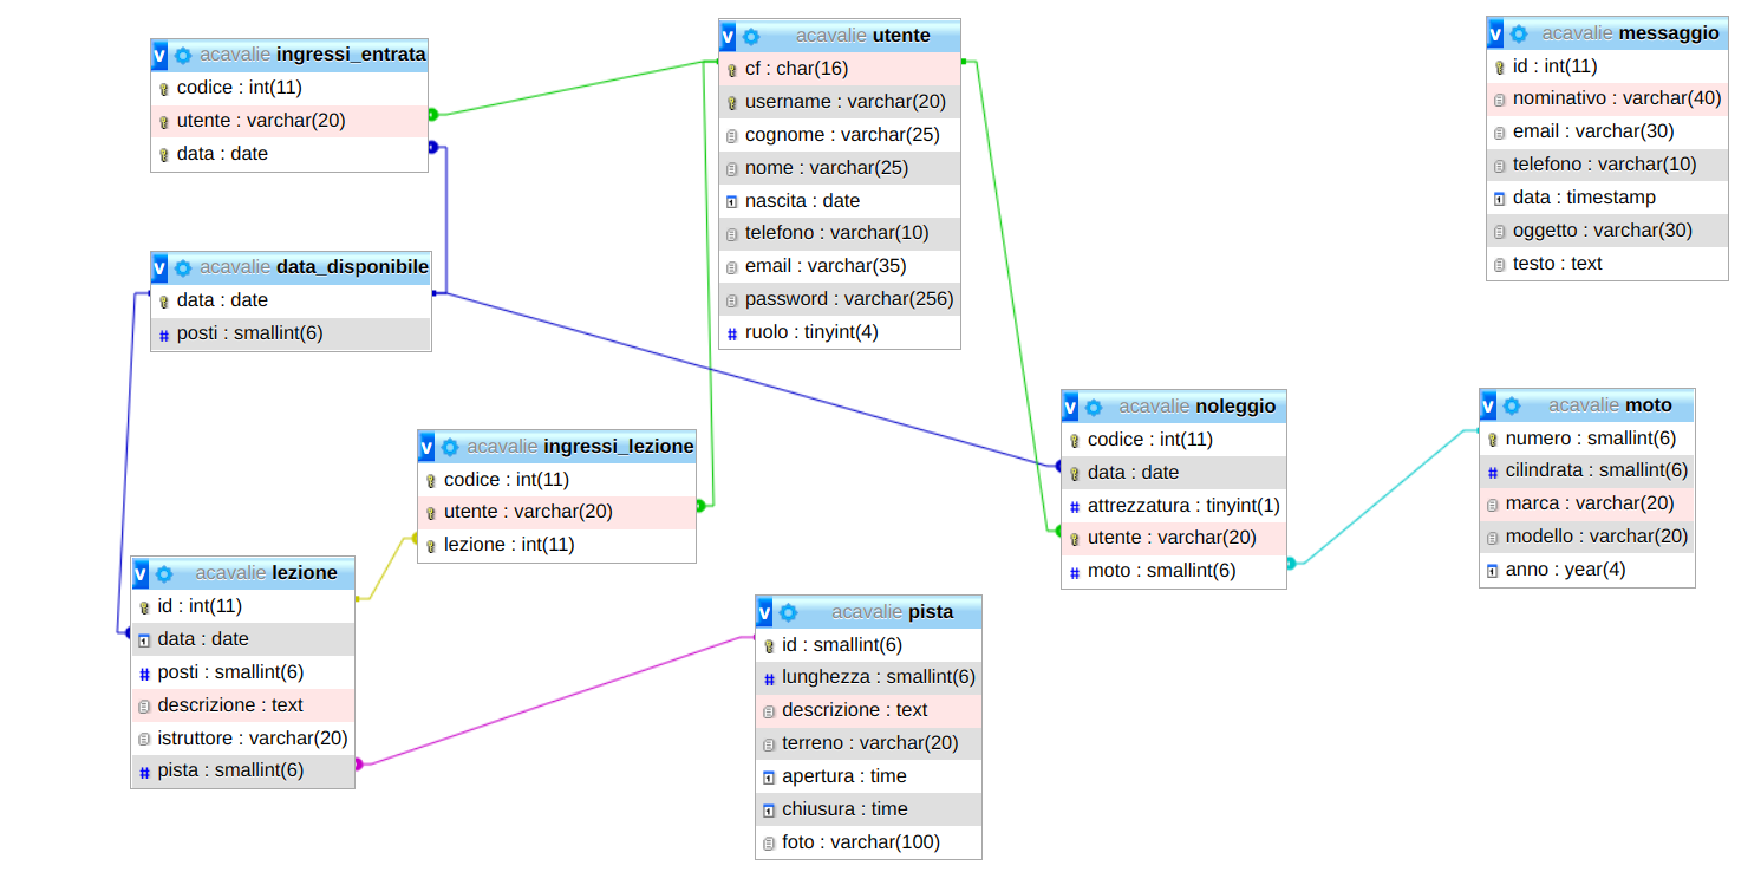
\includegraphics[scale=0.4]{./res/schemaSQL.pdf}
    \centering
    \caption{Schema SQL}
\end{figure}

	% 		\subsubsection{JavaScript}
	% 			Il linguaggio \textit{JavaScript} è stato utilizzato principalmente per due scopi.

Il primo riguarda la validazione dei form, i controlli sono stati fatti sia nella parte pubblica che nella parte privata (utente e admin). Per ogni pagina che necessitasse di una validazione di un form è stato creato il suo corrispondente file javascript (nomeValidation.js). Lo script analizza tutti gli input previsti per il form, controllandone la validità attraverso un'espressione regolare.
    
Il secondo, invece, è molto importante e utile per aggiornare costantemente il tipo di scelte che un utente può fare in base alle disponibilità dell'impianto. Vi sono infatti casi in cui le informazioni non possono essere rappresentate staticamente. Uno di questi casi riguarda la prenotazione di un ingresso o un corso da parte dell'utente. Viene data la possibilità all'utente di noleggiare una moto (l'attrezzatura non è un problema in questi casi) ed è quindi facile intuire che la disponibilità delle moto a noleggio varia di data in data (in base alle prenotazioni degli altri utenti).

Per poter costantemente aggiornare le moto disponibili in una giornata viene fatta una chiamata AJAX ad uno script PHP che, fornita una data di apertura, restituisce le moto ancora disponibili in quella data. Questa chiamata viene eseguita ogni volta che l'utente cambia la data in cui vuole prenotare l'ingresso o il corso.

Un altro caso simile accade nel form di prenotazione dei corsi, ma per una diversa motivazione. In questo caso si utilizza una chiamata AJAX per recuperare la descrizione del corso selezionato, evitando di costringere l'utente a muoversi tra le pagine per ricordare le informazioni del corso a cui si vuole prenotare. Questo, seppur non strettamente necessario, migliora l'esperienza utente e gli consente di portare a termine le operazioni in modo più rapido.
 
	% 		\subsubsection{XAMPP}
	% 			Per testare la parte dinamica del sito, in particolare le funzionalità lato server (PHP e SQL), il gruppo ha deciso di utilizzare XAMPP. Ciò ha reso possibile
anche testare il sito con dispositivi mobili, aprendo la porta 80 del proprio PC e rendendo il tutto accessibile nella rete locale.

Tramite questo il gruppo ha potuto testare il sito provando meglio i bottoni con le proprie dita, cosa che con lo strumento di ispezione di Chrome in modalità mobile era poco affidabile.
	% 		\subsubsection{Ispeziona di Chrome}
	% 			La modalità \textit{Ispeziona} del browser Chrome è buona per testare CSS e HTML, in quanto permette di visionare graficamente molti degli attributi dei fogli di stile, facilitando il debugging. Inoltre, permette di fare cambiamenti al CSS senza intaccare i file originali, consentendo di provare idee e metodologie di approccio di cui non si è particolarmente sicuri (come per esempio la scelta dei colori).
	% 	\subsection{Funzionamento generale}
	% 		Partiamo con il definire le 3 categorie di utenti:
\begin{itemize}
    \item Utente generico;
    \item Utente loggato;
    \item Amministratore.
\end{itemize}

Tutte le categorie di utenti possono visualizzare la parte pubblica del sito, ovvero le disponibilità e i servizi dell'impianto. È possibile inviare una richiesta di contatto tramite l'apposito form nella pagina \textit{"Contatti"} dell'area pubblica.\\

Il servizio di prenotazione richiede l'autenticazione dell'utente, il quale, se non è loggato durante la sessione, nel momento in cui clicca \textit{"Prenota Corso"} o \textit{"Prenota Ingresso"} verrà reindirizzato alla pagina
di autenticazione.
	% 		\subsubsection{Utente Generico}
	% 			L'utente generico è colui che deve ancora effettuare il login e dunque può navigare il sito vedendone solo la parte espositiva dello stesso.\\
Se non possiede un account, gli viene fornita la possibilità di crearne uno, tramite il form di registrazione. Una volta creato l'account può accedere all'area riservata, iniziando così ad usufruire dei servizi di prenotazione.\\
Chiaramente, se possiede un account e vuole usufruire dei servizi dell'utente autorizzato, può semplicemente fare l'accesso nell'area riservata. 
	% 		\subsubsection{Utente Autorizzato}
	% 			L'utente autorizzato è colui che ha effettuato l'accesso con le sue credenziali. Il suo stato gli permette di usare i servizi di prenotazione del sito. In particolare può:
\begin{enumerate}
    \item \textbf{Gestire gli ingressi personali}: prenotare un ingresso nuovo compilando l'apposito form (scegliendo data ed eventuale noleggio moto) oppure disdirne uno;
    
    \item \textbf{Gestire i corsi personali}: prenotare un corso compilando l'apposito form (scegliendo data ed eventuale noleggio moto) oppure disdirne uno;
    
    \item \textbf{Gestire i dati personali}: modificare i suoi dati personali (eccetto username ed e-mail).
\end{enumerate}
	% 		\subsubsection{Amministratore}
	% 			L'amministratore è colui che gestisce il sito e ha tutti i permessi.
In particolare può:
\begin{enumerate}
    \item \textbf{Gestire gli ingressi}: vedere le prenotazioni degli utenti, aggiungere nuove date (specificando la capacità massima), modificarle o cancellarle;
    
    \item \textbf{Gestire i noleggi}: aggiungere, togliere o modificare le moto e vedere le prenotazioni dei noleggi da parte degli utenti;
    
    \item \textbf{Gestire i tracciati}: aggiungere, togliere o modificare i tracciati;
    
    \item \textbf{Gestire i corsi}: aggiungere, togliere o modificare i corsi e vedere le prenotazioni da parte degli utenti;
    
    \item \textbf{Gestire i dati personali}: modificare i suoi dati personali (eccetto username ed e-mail);
    
    \item \textbf{Promuovere l'utenza}: promuove gli utenti ad admin (l'impianto assume constantemente personale);
    
    \item \textbf{Visualizzare i messaggi}: visualizzare i messaggi che arrivano dal form di contatto.
\end{enumerate}
	% 	\subsection{Intrusività}
	% 		Di seguito verrà descritto il livello di intrusività dei linguaggi rispetto al codice sorgente HTML:
\begin{itemize}
    \item \textbf{CSS}: \underline{non} intrusivo. Tutto il codice CSS è stato inserito in un file a parte, evitando del tutto pratiche come il CSS embedded o stili dichiari inline.
    
    \item \textbf{PHP}: \underline{non} intrusivo. Sebbene ci sia del codice HTML all'interno di alcuni file PHP, la corrispondente pagina HTML non contiene codice PHP. La motivazione per la quale c'è del codice HTML in file PHP è che spesso i dati, essendo dinamici, cambiano spesso in base ai dati inseriti da utente e amministratore. Quindi, per migliorare l'esperienza utente, non vengono visualizzate tabelle se non ci sono dati da mostrare o form se non ci sono possibilità che l'inserimento vada a buon fine. Un esempio è il caso in cui non ci sono informazioni sulle prenotazioni degli ingressi (per l'admin): non ha senso mostrare una tabella vuota all'utente, meglio stampare un messaggio di spiegazione. 
    
    \item \textbf{JavaScript}: \underline{non} intrusivo. Tutto il codice JavaScript è stato inserito in un file a parte. Tutti gli script, ad eccezione delle chiamate AJAX, aggiungono funzionalità non essenziali al sito, utili solamente a migliorare l'esperienza utente. Esempi sono la validazione dei form (vi è la validazione lato server) e il menu a scomparsa (senza JS il menu viene mostrato senza essere comprimibile).
\end{itemize}
		
	% \newpage

	\section{Validazione}
		Il controllo dell'accessibilità deve essere effettuato attraverso tool automatici, semiautomatici ma anche attraverso una validazione manuale.\\
É necessario ricordare come gli strumenti automatici non siano esaustivi ed il loro utilizzo non implica che il sito sia accessibile. Essi dunque possono essere utilizzati come strumento di supporto.\\
Per la validazione dell'accessibilità del sito si è deciso di utilizzare lo strumento \textit{\href{https://web.math.unipd.it/accessibility-dev/}{myWCAG4All}}. Il tool permette di avere un elenco di test esaustivo da effettuare, oltre alla possibilità di ottenere un report finale con i test effettuati e superati.\\
L'account utilizzato per tenere traccia dei test è: \textit{alecava41programmer@gmail.com}. All'interno dell'account è possibile trovare il sito "\textit{Adrenaline Motocross Park}" e i relativi test effettuati.\\
I tool utilizzati sono molteplici, in quanto ci si è attenuti alla guida che veniva data nel sito \textit{myWCAG4All} in relazione al test che si doveva effettuare. Quelli utilizzati principalmente sono stati:
\begin{itemize}
\setlength\itemsep{0em}
\item \href{https://wave.webaim.org/}{WAVE}.
\item \href{https://www.totalvalidator.com/}{Total Validator}.
\item \href{https://www.webfx.com/tools/read-able/}{Readability Test}.
\item \href{https://validator.w3.org/}{HTML Validator}.
\end{itemize}



 % anche vuoto
		\subsection{Strumenti usati}
			L'accessibilità, a livello di test automatici, è stata controllata tramite lo strumento WAVE Evaluation\footnote{\href{https://wave.webaim.org/}{Wave Evaluation}}.\\
			\subsubsection{WAVE Evaluation}
				% Questo tool ha permesso al gruppo di trovare alcuni problemi legati all'accessibilità dei contenuti. Esso ha individuato alcune problematiche rispetto al tipo di attributi \textit{aria} utilizzati e rispetto alla lunghezza dell'\textit{alt} di alcune immagini. Sebbene abbia individuato dei falsi negativi è stato utile per raffinare alcuni aspetti dell'accessibilità. È stato utilizzato anche per i test sul contrasto dei colori utilizzati.
Questo tool ha permesso al gruppo di trovare alcuni problemi legati all'accessibilità dei contenuti. Esso ha individuato alcune problematiche rispetto al tipo di attributi \textit{aria} utilizzati e rispetto alla lunghezza dell'\textit{alt} di alcune immagini. Sebbene abbia individuato dei falsi negativi è stato utile per raffinare alcuni aspetti dell'accessibilità. È servito anche per i test sul contrasto dei colori utilizzati.\\
Qui di seguito vengono messi alcuni screenshot che ne evidenziano l'utilità.
			% \subsubsection{W3C HTML Validator}
			% 	Lo strumento di validazione di W3C ci ha consentito di validare anche l’HTML prodotto dalle pagine PHP, poichè permette di incollare direttamente il codice HTML prodotto dallo script. È il motivo per cui è stato utilizzato per validare tutto il codice HTML. 

Non è stato possibile testare tutte le possibili combinazioni degli esiti degli script PHP (richiedeva la presenza di situazioni complesse da simulare). Per questo motivo, oltre al tool indicato, è stata effettuata la verifica manuale in stile \textit{walkthrough} degli script PHP, controllando che tutti i testi aggiunti dinamicamente venissero inclusi nei corretti tag.
			% \subsubsection{W3C CSS Validator}
			% 	Abbiamo utilizzato il servizio di validazione CSS del W3C così da assicurare in modo rigoroso il rispetto dello standard.
			% \subsubsection{PhpCodeChecker}
			% 	Attraverso l’utilizzo di questo tool è stata verificata la sintassi di tutti i file PHP. Il tool faceva anche un controllo soft su errori comuni (non sintattici). È stato molto utile, essendo il sito composto principalmente da pagine dinamiche.
			% \subsubsection{Esprima}
			% 	Tramite l’utilizzo di questo strumento è stata controllata la sintassi di tutti gli script JavaScript utilizzati per la validazione dei campi lato client, le chiamate AJAX e la gestione della scomparsa del menu.
			% \subsubsection{Screenshot}
			% 	% input degli screenshot messi nella cartella res
				
	\newpage

	% \section{Organizzazione del lavoro}
	% 	Il lavoro del progetto \textit{Adrenaline Motocross Park} è stato suddiviso nel seguente modo:
\begin{itemize}
    \item \textbf{Brugnolaro Filippo}:
        \begin{itemize}
            \item[$\circ$] Parte dei file HTML della parte pubblica;
            \item[$\circ$] Maggior parte dei file Javascript;
            \item[$\circ$] Validazione HTML e Javascript;
            \item[$\circ$] Prova con screen reader;
            \item[$\circ$] Stesura della relazione.
        \end{itemize}
    \item \textbf{Cavaliere Alessandro}:
        \begin{itemize}
            \item[$\circ$] File HTML della parte privata dell'amministratore;
            \item[$\circ$] Maggior parte dei file PHP della parte privata dell'amministratore;
            \item[$\circ$] Parte dei file Javascript;
            \item[$\circ$] Parte del database SQL;
            \item[$\circ$] Parte dei file CSS.
        \end{itemize}
    \item \textbf{Gambirasio Leonardo}:
        \begin{itemize}
            \item[$\circ$] Parte dei file HTML della parte pubblica;
            \item[$\circ$] Parte dei file PHP;
            \item[$\circ$] Parte dei file CSS;
            \item[$\circ$] Validazione CSS;
            \item[$\circ$] Test dei browser.
        \end{itemize}
    \item \textbf{Simionato Riccardo}:
        \begin{itemize}
            \item[$\circ$] File HTML della parte priva dell'utente;
            \item[$\circ$] Maggior parte dei file PHP della parte privata dell'utente;
            \item[$\circ$] Parte del database SQL;
            \item[$\circ$] Parte dei file CSS;
            \item[$\circ$] Validazione dei file PHP.
        \end{itemize}
\end{itemize}
	
	% \newpage
	
	\appendix
	\addcontentsline{toc}{part}{Appendice}
	\section{Note per la correzione}
		In questa sezione vengono illustrate alcune informazioni utili per i valutatori.
Sottolineiamo che il link illustrato in prima pagina funziona solo se viene creato correttamente un tunnel verso
\textit{caa.studenti.math.unipd.it}.
		\subsection{Credenziali}
			Vengono fornite le credenziali dell’account amministratore:
\begin{itemize}
    \item Username: \textit{admin}
    \item Password: \textit{admin}
\end{itemize}
Vengono fornite le credenziali dell’account utente:
\begin{itemize}
    \item Username: \textit{user}
    \item Password: \textit{user}
\end{itemize}
É in ogni caso sempre possibile creare nuovi utenti tramite l'apposito form di registrazione.
		\subsection{Popolamento}
			Per avere una reale presentazione del sito, sono già stati inseriti alcuni record: date di apertura, corsi, tracciati, moto noleggiabili, prenotazioni ingressi/corsi, messaggi.\\
I dati inseriti non devono per forza corrispondere con la realtà e pertanto non devono essere considerati come difetti del sito.
		% \subsection{Visibilità}
		% 	A causa dell'utilizzo di icone soggette a copyright che ne permette l'uso esclusivamente personale, il sito non può essere in alcun modo visibile al pubblico.

    
\end{document}